\section[Proof Discharge Algorithm]{Proof Discharge Algorithm through Illustative Examples}
\label{sec:examples}
This chapter demonstrates our proof discharge algorithm through examples.
We consider proof obligations generated due to invariants shown in \cref{tab:llproductInv,fig:llTraverseProductInv}.

\subsection{Properties of Proof Discharge Algorithm}
\label{sec:algoprops}
An algorithm that evaluates the truth value of a proof obligation is called a
{\em proof discharge algorithm}.
In case a proof discharge algorithm deems a proof obligation to be unprovable,
it is expected to return {\em false} with a set of counterexamples that falsify
the proof obligation.
A proof discharge algorithm is {\em precise} if for all proof obligations,
the truth value evaluated by the algorithm is identical to the proof obligation's
{\em actual} truth value.
A proof discharge algorithm is {\em sound} if:
(a) whenever it evaluates a proof obligation to true,
the actual truth value of that proof obligation is also true,
and (b) whenever it generates a counterexample, that counterexample
must falsify the proof obligation.
However, it is possible for a sound proof discharge algorithm to return false
(without counterexamples) when the proof obligation was actually provable.

For proof obligations generated by our equivalence checker procedure,
it is always safe for a proof discharge algorithm to return false (without counterexamples).
Keeping this in mind, our proof discharge algorithm is designed to be {\em sound}.
Conservatively evaluating a proof obligation to false (when it was actually provable)
may prevent the equivalence proof from completing successfully.
However, importantly, the overall equivalence procedure remains sound i.e.
(a) either it successfully finds a valid proof of equivalence (bisimulation relation)
or (b) it conservatively returns {\em unknown}.

Resolving the truth value of a proof obligation that contains a \recursiveRelation{}
such as $\sv{l} \indEq{} \lifted{list}{\mem{}}{lnode}{\cv{l}}$ is unclear.
Fortunately, the shapes of the proof obligations generated by our equivalence
checker are restricted.
Our equivalence checking algorithm ensures that, for an invariant
$\phi_s=({\tt \phi^{1}_s \land \phi^{2}_s \land ... \land \phi^{k}_s})$,
at any node $s$ of a product-CFG,
if a \recursiveRelation{} appears in $\phi_s$, it
must be one of $\phi^{1}_s$, $\phi^{2}_s$, ..., or $\phi^{k}_s$. We call
this the {\em conjunctive \recursiveRelation{}} property of an invariant $\phi_s$.

A proof obligation
$\hoareTriple{\phi_s}{e}{\phi_d}$, where $e=(\rho_S,\rho_C)$,
gets lowered using
${\tt WP}_{e}(\phi_d)$ (as shown in \cref{eqn:firstOrderFormula}) to a first-order logic formula of the following form:

\begin{equation}
\label{eqn:proofObligationShape}
(\eta^{l}_1 \land \eta^{l}_2 \land ... \land \eta^{l}_m) \Rightarrow (\eta^{r}_1 \land \eta^{r}_2 \land ... \land \eta^{r}_n)
\end{equation}

Thus, due to the conjunctive \recursiveRelation{} property of $\phi_s$ and $\phi_d$, any
\recursiveRelation{} in \cref{eqn:proofObligationShape} must appear as
one of $\eta^{l}_i$ or $\eta^{r}_j$.
To simplify proof obligation discharge,
we break a first-order logic proof obligation $P$ of the form in \cref{eqn:proofObligationShape}
into multiple smaller proof obligations
of the form
$P_j:(\lhs{} \Rightarrow{\tt \eta^{r}_j})$, for $j=1..n$. Each proof obligation
$P_j$ is then discharged separately.  We call this conversion from
a bigger query to multiple smaller queries, {\em \rhs{}-breaking}.

We provide a sound (but imprecise) proof discharge algorithm that converts
a proof obligation generated by our equivalence checker into a series
of SMT queries.
Our algorithm begins by categorizing a proof obligation into
one of three types; each type is discussed separately in subsequent
sections.
The categorization is based on an `iterative unification and rewriting' procedure,
which we describe next.
We use an {\em unroll parameter} $k$ for our categorization.

\subsection{Iterative Unification and Rewriting Procedure}
\label{sec:unifyandrewrite}
We begin with some definitions.
An expression $e$ whose top-level constructor is a lifting
constructor, e.g., $e=\lifted{list}{\mem{}}{lnode}{\cv{l}}$,
is called a {\em lifted expression}.
An expression $e$ of the form \prodAccess{v}{a_1,a_2,.,a_n} i.e.
a variable with {\em zero} or more {\em accessor}-operators applied on it,
is called a {\em pseudo-variable}.
Note that, a variable $v$ is a pseudo-variable.
An expression $e$ in which (a) all accessors (e.g., `\prodAccess{\_}{tail}') appear
in a pseudo-variable and (b) each {\em is}-operator (e.g., `\sumIs{\_}{LCons}') operate
on a pseudo-variable, is called a {\em canonical expression}.

Consider the expression tree of a canonical expression $e$.
The internal nodes of $e$ represents ADT value constructors and
the \sumDtor{} sum-deconstruction operator.
The leaves of $e$ (also called {\em atoms} of $e$) are the
pseudo-variables (of scalar and ADT type),
the scalar expressions (of \type{Unit}, \type{Bool} and \type{i<N>} types),
and lifted expressions.

The {\em expression path} to a node $v$ in $e$'s tree is the path from the root
of $e$ to the node $v$.
The {\em expression path condition} represents the conjunction of all the \underline{\tt if}
conditions (if the \underline{\tt then} branch of taken along the path), or their
negation (if the \underline{\tt else} branch is taken along the path).
For example, in the expression \sumIf{c} \sumThen{a} \sumElse{b},
the expression path condition of $c$ is {\tt true}, of $a$ is $c$,
and of $b$ is $\neg c$.

When we attempt to unify two expressions, we unify the
structures created by the ADT value constructors and
the \sumDtor{} operator of their canonical forms.
The unification procedure either fails to unify, or it
returns tuples $(p_1,p_2,a_1,e_2)$ where atom $a_1$
at expression path condition $p_1$ in one expression is correlated
with expression $e_2$ at expression path condition $p_2$ in the other expression.

For two non-atomic expressions, $e_1$ and $e_2$ to unify successfully,
it must be true that either the top-level constructor in $e_1$ and $e_2$ is
the same value constructor (in which case an unification is attempted for each
of their children),
{\em or} the top-level constructor in one of $e_1$ or $e_2$ is \sumDtor{}.

If the top-level constructor of exactly one of $e_1$ and $e_2$ (say $e_1$)
is \sumDtor{}, then $e_2$ must have a value constructor at its root.
In such a case, we {\em rewrite} $e_2$ using \sumDtor{} such that
one of the branches contain $e2$ under the condition {\em true}
and all other branches have a {\em false} condition.
the condition of the branch containing $e_2$ is {\em true}
while all other branches have a {\em false} condition.
For example, we can rewrite $\cons{LCons}(e_1, e_2)$ to \sumIf{false} \sumThen{\cons{LNil}}
\sumElse{\cons{LCons}(e_1,e_2)}.
Next, we unify each child (condition and branch expressions) of the top-level
\sumDtor{} operators of (possibly rewritten) $e_1$ and $e_2$.
Whenever we descend down an \sumDtor{} operator, we keep track of
the expression path conditions for both expressions.
Recall that the \sumDtor{} operator for an ADT $T$ must have exactly one branch
for each value constructor of $T$.
Moreover, the branch associated with the value constructor $V$ must contain
an expression whose top-level constructor is $V$.

If one of $e_1$ and $e_2$ (say $e_2$) is atomic,
unification always succeeds and returns $(p_2,p_1,e_2,e_1)$
With each atom of an ADT type, we associate an {\em unrolling procedure}
By definition, an ADT atom is either a pseudo-variable of a lifted expression.
Every (pseudo-)variable is associated with its unrolling procedure governed by its ADT.
For example, the unrolling procedure for \type{List} variable $l$ is $U_S$ (\cref{eqn:specDeconstruct}).
For lifted expressions, the unrolling procedure is given by the
its definition, e.g., $U_C$ (\cref{eqn:clist}) for the lifting constructor \lift{list}{}{lnode}.

Given two expressions $e_a$ and $e_b$ at expression path conditions $p_a$ and $p_b$
respectively, an {\em iterative unification and rewriting procedure}
$\Theta(e_a,e_b,p_a,p_b)$ is used to identify a set of correlation tuples
between the atoms in the two expressions.
This iterative procedure begins with an attempt to unify $e_a$ and $e_b$.
If this unification fails, we return a failure for the original expressions $e_a$ and $e_b$.
Else, we obtain correlation tuples between atoms and expressions
(with their expression path conditions).
If the unification correlates an atom $a_1$ at expression path condition $p_1$
with another atom $a_2$ at expression path condition $p_2$, we add
$(p_1,a_1,p_2,a_2)$ to the final output.
Otherwise, if the unification correlates an atom $a_1$ at expression path condition $p_1$
to a non-atomic expression $e_2$ at expression path condition $p_2$,
we {\em rewrite} $a_1$ using its unrolling procedure to obtain expression $e_1$.
The unification algorithm then proceeds by unifying $e_1$ and $e_2$ through
a recursive call to $\Theta(e_1,e_2,p_1,p_2)$.
The maximum number of rewrites performed by $\Theta(e_a,e_b,p_a,p_b)$ (before termination)
is upper bounded by the sum of number of ADT value constructors in $e_a$ and $e_b$.

For a \recursiveRelation{} $l_1 \indEq{} l_2$, we unify $l_1$ and $l_2$ through a
call to $\Theta(l_1,l_2,true,true)$.
If the $n$ tuples obtained after a successful unification are $(p_1^i,a_1^i,p_2^i,a_2^i)$
(for $i=1\ldots n$), then the {\em decomposition} of $l_1 \indEq{} l_2$ is defined as:

\begin{equation}
\label{eqn:decompose}
l_1 \indEq{} l_2 \Leftrightarrow \bigwedge \limits_{i=1}^n (p_1^i \land p_2^i \rightarrow (a_1^i = a_2^i))
\end{equation}

For example, the unification of `\sumIf{c_1} \sumThen{\cons{LNil}} \sumElse{\cons{LCons}(0,l_1)}'
and `\sumIf{c_2} \sumThen{\cons{LNil}} \sumElse{\cons{LCons}(i, \lifted{list}{\mem{}}{lnode}{l_2})}'
yields the correlation tuples: $(true,true,c_1,c_2)$, $(\neg c_1, \neg c_2, 0, i)$ and
$(\neg c_1, \neg c_2, l_1, \lifted{list}{\mem{}}{lnode}{l_2})$.
Hence, the \recursiveRelation{} ``\sumIf{c_1} \sumThen{\cons{LNil}} \sumElse{\cons{LCons}(0,l_1)} \indEq{}
\sumIf{c_2} \sumThen{\cons{LNil}} \sumElse{\cons{LCons}(i, \lifted{list}{\mem{}}{lnode}{l_2})}''
decomposes into $(c_1 = c_2) \land (\neg c_1 \land \neg c_2 \rightarrow 0 = i)
\land (\neg c_1 \land \neg c_2 \rightarrow l_1 \indEq{} \lifted{list}{\mem{}}{lnode}{l_2})$.
Similarly, the decomposition of $l_1 \indEq{} \cons{LCons}(42, \lifted{list}{\mem{}}{lnode}{l_2})$ is given by
$(\sumIs{l_1}{LCons}) \land (\sumIs{l_1}{LCons} \rightarrow \prodAccess{l_1}{val}=42)
\land (\sumIs{l_1}{LCons} \rightarrow \prodAccess{l_1}{next} \indEq{} \lifted{list}{\mem{}}{lnode}{l_2})$.
In case of a failed unification, the {\em decomposition} is defined to be {\em false},
e.g., $\cons{LNil} \indEq{} \cons{LCons}(0, l)$ decomposes into $false$.

Each conjunctive clause of the form $(p_1^i \land p_2^i \rightarrow (a_1^i = a_2^i))$\footnote{
If $a_1^i$ and $a_2^i$ are ADT values, then we replace $a_1^i = a_2^i$ with $a_1^i \indEq{} a_2^i$.}
in the decomposition is called a {\em decomposition clause}.
A decomposition clause may relate only atomic values, i.e.,
it may relate either (a) two scalars or (b) two ADT variable(s) and/or lifted expression(s).
However, we restrict \recursiveRelation{} invariants to a shape such that each
\recursiveRelation{} in its decomposition strictly relates ADT values to lifted expressions only.
This is discussed in more detail along with all other invariant shapes in \cref{sec:invinference}.
We {\em decompose} a \recursiveRelation{} by replacing it with its decomposition.
We {\em decompose} a proof obligation $P$ to $P_D$ by decomposing all \recursiveRelations{} in $P$.

\subsection{Categorization of Proof Obligations}
We {\em unroll a \recursiveRelation{} $l_1 \indEq{} l_2$} by rewriting the
top-level expressions $l_1$ and $l_2$ through their unrolling procedures (if possible)
and decomposing it.
We {\em unroll an expression $e$} by unrolling each \recursiveRelation{} in $e$.
More generally, the $k$-unrolling of $e$ is found by unrolling the $(k-1)$-unrolling
of $e$ recursively.
For a decomposed proof obligation $P_D:\lhs{} \Rightarrow \rhs{}$, we identify its $k$-unrolling (say $P_K$),
where $k$ is a fixed parameter called the {\em unrolling parameter}.
After $k$-unrolling, we {\em eliminate} those decomposition clauses $(p_1 \land p_2 \rightarrow (a_1 = a_2))$
in $P_K$ whose $(p_1 \land p_2)$ evaluates to false under \lhs{} ignoring all \recursiveRelations{},
yielding an equivalent proof obligation, say $P_E$.
For example, the one-unrolling of $P: \lhs{} \Rightarrow l \indEq{} \lifted{list}{\mem{}}{lnode}{0}$,
after elimination, yields $P_E: \lhs{} \Rightarrow \sumIs{l}{LNil}$.
We categorize a proof obligation $P: \lhs{} \Rightarrow \rhs{}$ based on the $k$-unrolled form
of its decomposition (i.e. $P_E$) as follows:

\begin{itemize}
\item Type I: $P_E$ does not contain \recursiveRelations{}
\item Type II: $P_E$ contains \recursiveRelations{} {\em only} in the \lhs{}
\item Type III: $P_E$ contains \recursiveRelations{} in the \rhs{}
\end{itemize}

The categorization method is {\em sound} as long as the elimination of decomposition
clauses is sound (but possibly not precise).
In other words, it is possible that we are unable to eliminate a \recursiveRelation{} in $P_K$,
due to an imprecise algorithm for elimination of decomposition clauses.
However, our proof discharge algorithm remains sound irrespective of such imprecision
during categorization.
Henceforth, we will simply use $k$-unrolling of $P$ to refer to $P_E$ directly.
Next, we describe the algorithm for each type of proof obligations
in \cref{sec:cat1,sec:cat2,sec:cat3}.

\subsection{Handling Type I Proof Obligations}
\label{sec:cat1}
In \cref{fig:llAllocProductCFG}, consider a proof obligation generated
across the product-CFG edge \scedge{0}{0}{3}{3}
while checking if the {\circled{\footnotesize I4}} invariant in \cref{tab:llproductInv},
$\sv{l} \indEq{} \lifted{list}{\mem{}}{lnode}{\cv{l}}$ holds at (\scpc{3}{3}):
\hoareTriple{\scpcinv{0}{0}}{\spath{0,3},\cpath{0,3}}{\sv{l} \indEq{} \lifted{list}{\mem{}}{lnode}{\cv{l}}}.
The precondition $\scpcinv{0}{0} \equiv (\sv{n} = \cv{n})$ does not contain a \recursiveRelation{}.
When lowered to first-order logic through {\tt WP}$_{\spath{0,3},\cpath{0,3}}$, this translates to
$\sv{n} = \cv{n} \Rightarrow \cons{LNil} \indEq{} \lifted{list}{\mem{}}{lnode}{0}$.
Here, \cons{LNil} is obtained for \sv{l} and {\tt 0} (null) is obtained for \cv{l}.
The one-unrolled form of this proof obligation yields
$\sv{n} = \cv{n} \Rightarrow \cons{LNil} \indEq{} \cons{LNil}$ which trivially resolves to true.

Consider the following example of a proof obligation:
\hoareTriple{\scpcinv{0}{0}}{\spath{0,3,5,3},\cpath{0,3}}{\sv{l} \indEq{} \lifted{list}{\mem{}}{lnode}{\cv{l}}}.
Notice, we have changed the path in $S$ (with CFG \cref{fig:llAllocSpecIRCFG}) to \spath{0,3,5,3} here.
In this case, the corresponding first-order logic formula evaluates to:
$\sv{n} = \cv{n} \land 0 <_u \sv{n} \Rightarrow \cons{LCons}(0, \cons{LNil}) \indEq{} \lifted{list}{\mem{}}{lnode}{0}$.,
where $(0 <_u \sv{n})$ is the path condition for the path \spath{0,3,5,3}.
One-unrolling of this proof obligation converts \lifted{list}{\mem{}}{lnode}{0} to \cons{LNil} and
decomposes \rhs{} into false due to failed unification of \cons{LCons} and \cons{LNil}.
The proof obligation is further discharged using an SMT solver
which provides a counterexample (model) that evaluates the
formula to false. For example, the counterexample $\{ \mapping{\sv{n}}{42}, \mapping{\cv{n}}{42} \}$
evaluates this formula to false.
These counterexamples assist in faster convergence of our correlation search and invariant inference procedures
(as we will discuss later in \cref{sec:searchalgo,sec:invinference}).

Thus for type I queries, $k$-unrolling reduces all \recursiveRelations{}
in the original proof obligation into scalar equalities.
The resulting query is further discharged using an SMT solver.
Please refer to \cref{sec:smtencoding,sec:cerecons} for the intricacies
of (a) translation of the formula to SMT logic and
(b) reconstruction of counterexamples from the models returned by the SMT solver.
Assuming a capable enough SMT solver,
all proof obligations in type I can be discharged precisely, i.e., we can always
decide whether the proof obligation evaluates to true or false.
If it evaluates to false, we also obtain counterexamples.

\subsection{Handling Type II Proof Obligations}
\label{sec:cat2}
Consider the proof obligation originating due to \circled{\small I2} invariant $\sv{sum} = \cv{sum}$
across edge \scedge{2}{2}{2}{2} in \cref{fig:llTraverseProduct}:
\hoareTriple{\scpcinv{2}{2}}{\spath{2,5,2}, \cpath{2,4,2}}{\sv{sum} = \cv{sum}}, where
the node invariant \scpc{2}{2} contains the \recursiveRelation{} $\sv{l} \indEq{} \lifted{list}{\mem{}}{lnode}{\cv{l}}$.
The corresponding (simplified) first-order logic formula for this proof obligation is:
$(\sv{l} \indEq \lifted{list}{\mem{}}{lnode}{\cv{l}} \land \sv{sum} = \cv{sum} \land \sumIs{\sv{l}}{LCons} \land \cv{l}\neq0) \Rightarrow (\sv{sum} + \prodAccess{\sv{l}}{val}) = (\cv{sum} + \structPointer{\cv{l}}{\mem{}}{lnode}{val})$.
We fail to remove the \recursiveRelation{} on the \lhs{} even after
$k$-unrolling for any finite unrolling parameter $k$ because both sides of \indEq{}
represent list values of arbitrary length.
In such a scenario, we do not know of an efficient
SMT encoding for the \recursiveRelation{} $\sv{l} \indEq{} \lifted{list}{\mem{}}{lnode}{\cv{l}}$.
Ignoring this \recursiveRelation{} will incorrectly (although soundly) evaluate
the proof obligation to false; however, for a successful equivalence
proof, we need the proof discharge algorithm to evaluate it to true. Let's call this
requirement \circled{\footnotesize R1}.

Now, consider the proof obligation formed by correlating two iterations
of the loop in program $S$ (with CFG \cref{fig:llTraverseSpecCFG}) with
one iteration of the loop in program $C$ (with CFG \cref{fig:llTraverseCCFG}):
\hoareTriple{\scpcinv{2}{2}}{\spath{2,5,2,5,2}, \cpath{2,4,2}}{\sv{sum} = \cv{sum}}.
The equivalent first-order logic formula is:
$\sv{l} \indEq{} \lifted{list}{\mem{}}{lnode}{\cv{l}} \land \sv{sum} = \cv{sum} \land \sumIs{\sv{l}}{LCons} \land \sumIs{\prodAccess{\sv{l}}{tail}}{LCons} \Rightarrow (\sv{sum} + \prodAccess{\sv{l}}{val} + \prodAccess{\sv{l}}{tail,val}) = (\cv{l} + \structPointer{\cv{l}}{\mem{}}{lnode}{val})$.
Similar to the prior proof obligation, its equivalent first-order logic formula contains a \recursiveRelation{} in the \lhs{}.
Clearly, this proof obligation should evaluate to false.
Whenever a proof obligation evaluates to false, we
expect an ideal proof discharge algorithm to generate
counterexamples that falsify the proof obligation.
Let's call this requirement \circled{\footnotesize R2}.
Recall that these counterexamples help in faster
convergence of our correlation search and invariant inference procedures.

To tackle requirements \circled{\footnotesize R1} and \circled{\footnotesize R2},
our proof discharge algorithm converts the original proof obligation $P: \hoareTriple{\phi_s}{e}{\phi_d}$
into two approximated proof obligations $(P_{pre-o}: \hoareTriple{\phi^{o_{d_1}}_s}{e}{\phi_d})$
and $(P_{pre-u}: \hoareTriple{\phi^{u_{d_2}}_s}{e}{\phi_d})$.
Here $\phi^{o_{d_1}}_s$ and $\phi^{u_{d_2}}_s$ represent the over- and under-approximated
versions of precondition $\phi_s$ respectively, and $d_1$ and $d_2$ represent
{\em depth parameters} that indicate the degree of over- and under-approximation.
To explain our over- and under-approximation scheme, we
first introduce the notion of {\em depth of an ADT value}.

\subsubsection{Depth of ADT Values}
To define the depth of an ADT value $v$, we view the value as a tree $\mathcal{T}(v)$.
This tree representation is similar to the one briefly introduced in \cref{sec:unifyandrewrite}.
The internal nodes of $\mathcal{T}(v)$ represent ADT value constructors and
the leafs (also called {\em terminals}) represent scalar values (i.e. boolean and bitvector literals).
The depth of a value constructor or a scalar in $v$ is simply the depth of
its associated node in $\mathcal{T}(v)$.
The {\em depth of ADT value $v$} is defined as the depth of $\mathcal{T}(v)$.
For example, the depth of $\cons{LCons}(1, \cons{LCons}(4, \cons{LNil}))$ is {\tt 2},
where as the depth of the literal {\tt 1} is {\tt 1}.
\Cref{fig:adttrees} shows the tree representation and depths for different values.

\subsubsection{Overapproximation and Underapproximation of Recursive Relations}
The $d$-depth overapproximation of a \recursiveRelation{} $l_1 \indEq{} l_2$,
denoted by $l_1 \indEqDepth{d} l_2$, represents the condition that
$l_1$ and $l_2$ are {\em recursively equal up to depth $d$}. i.e.,
$l_1$ and $l_2$ have identical structures and all
{\em terminals} at depths $\leq d$ in the trees of both values
are equal (under the precondition that the terminals exist);
however, terminals at depths $>d$ may have different values.
$l_1 \indEqDepth{d} l_2$ (for finite $d$) is a weaker
condition than $l_1 \indEq{} l_2$ (i.e. overapproximation).
The true equality i.e. $l_1 \indEq{} l_2$ can be thought of as equality of structures
and all terminals up to an unbounded depth i.e. $l_1 \indEqDepth{\infty} l_2$.

The $d$-depth underapproximation of a \recursiveRelation{} $l_1 \indEq{} l_2$
is written as $l_1 \indEqUapprox{d} l_2$, where $\indEqUapprox{d}$ represents
the condition that $l_1$ and $l_2$ are {\em recursively equal and bounded to depth $d$},
i.e., $l_1$ and $l_2$ have a maximum depth $\leq d$ {\em and}
they are recursively equal up to depth $d$.
Thus, $l_1 \indEqUapprox{d} l_2$ is equivalent to
$(\depthBound{d}{l_1} \land \depthBound{d}{l_2} \land l_1 \indEqDepth{d} l_2)$,
where $\depthBound{d}{l}$ represents the condition that the maximum
depth of $l$ is $d$.
$l_1 \indEqUapprox{d} l_2$ (for finite $d$) is a stronger condition than
$l_1\indEq{}l_2$ (i.e. underapproximation)
as it bounds the depth to $d$ while also ensuring equality till depth $d$.
For arbitrary depths $a$ and $b$ ($a \leq b$),
the approximations of $l_1 \indEq{} l_2$ are related as follows:

\begin{equation}
\label{eqn:approxrels}
l_1 \indEqUapprox{a} l_2 \Rightarrow l_1 \indEqUapprox{b} l_2 \Rightarrow l_1 \indEq{} l_2 \Rightarrow l_1 \indEqDepth{b} l_2 \Rightarrow l_1 \indEqDepth{a} l_2
\end{equation}

\subsubsection{SMT Encoding of Approximate Recursive Relations}
Unlike the original \recursiveRelation{} $l_1 \indEq{} l_2$,
its approximations $l_1\indEqDepth{d}l_2$ and $l_1\indEqUapprox{d}l_2$ can be encoded in SMT logic as shown below:

\begin{itemize}
\item $l_1 \indEqDepth{d} l_2$ is equivalent to the condition that
the tree structures of $l_1$ and $l_2$ are isomorphic till depth $d$ {\em and}
the corresponding terminal values in both $d$-depth isomorphic structures are also equal.
Note that these conditions only require scalar equalities.
$l_1 \indEqDepth{d} l_2$ can be identified through a {\em $d$-depth bounded} iterative unification and rewriting
procedure described in \cref{sec:unifyandrewrite}.
In this modified algorithm, We eagerly expand both expressions through rewriting and collect all correlation
tuples till depth $d$.
Finally, we only keep those correlation tuples that relate scalar values and discard the \recursiveRelations{}.

For example, the condition $l \indEqDepth{1} \lifted{list}{\mem{}}{lnode}{p}$ is computed
through iterative unification and rewriting till depth one; yielding the correlation tuples:
$(true, true, \sumIs{l}{LNil}, p = 0)$, $(\sumIs{l}{LCons} ,p \neq 0, \prodAccess{l}{val} = \structPointer{p}{\mem{}}{lnode}{val})$
and $(\sumIs{l}{LCons}, p \neq 0, \prodAccess{l}{tail} = \lifted{list}{\mem{}}{lnode}{\structPointer{p}{\mem{}}{lnode}{next}})$.
Keeping only those correlation tuples that relate scalar expressions, the above condition
reduces to the SMT-encodable predicate:
$$
(\sumIs{l}{LNil}) = (p = 0) \land \sumIs{l}{LCons} \land (p \neq 0) \rightarrow \prodAccess{l}{val} = \structPointer{p}{\mem{}}{lnode}{val}
$$

\item Recall that $l_1 \indEqUapprox{d} l_2 \equiv (\depthBound{d}{l_1} \land \depthBound{d}{l_2} \land l_1 \indEqDepth{d} l_2)$.
$\depthBound{d}{l}$ is equivalent to the condition that the tree nodes at depths $>d$ are unreachable.
This is achieved through expanding $l$ through rewriting till depth $d$ and asserting the unreachability
of \sumDtor{} paths that reach nodes with depths $>d$ (i.e. the negation of their expression path conditions).
For example, for a \type{List} variable $l$, the condition $\depthBound{2}{l}$ is equivalent to
$\sumIs{l}{LNil} \vee (\sumIs{l}{LCons} \land \sumIs{\prodAccess{l}{tail}}{LNil})$.
Similarly, $\depthBound{2}{\lifted{list}{\mem{}}{lnode}{p}}$ is equivalent to
$(p = 0) \vee (p \neq 0 \land \structPointer{p}{\mem{}}{lnode}{next} = 0)$.
Finally, $l \indEqUapprox{2} \lifted{list}{\mem{}}{lnode}{p} \Leftrightarrow \depthBound{2}{l}
\land \depthBound{2}{\lifted{list}{\mem{}}{lnode}{p}} \land l \indEqDepth{2} \lifted{list}{\mem{}}{lnode}{p}$.
\end{itemize}

\subsubsection{Summary of Type II Proof Discharge Algorithm}
\label{cat2summary}
We over- (under-) approximate a precondition $\phi$ till depth $d$ by $d$-depth over- (under-) approximating
each \recursiveRelation{} occuring in $\phi$.
Due to the conjunctive \recursiveRelation{} property (\cref{sec:algoprops}),
the over- and under-approximation of $\phi$ are also weaker and stronger conditions compared to $\phi$
respectively.
For a type II proof obligation $P: \hoareTriple{\phi_s}{e}{\phi_d}$, we first
submit the proof obligation $(P_{pre-o}: \hoareTriple{\phi^{o_{d_1}}_s}{e}{\phi_d})$
to the SMT solver. Recall that the precondition $\phi^{o_{d_1}}_s$
is the $d_1$-depth overapproximated version of $\phi_s$.
If the SMT solver evaluates $P_{{pre-o}}$ to true, then we return true for
the original proof obligation $P$ --- if the
Hoare triple with an overapproximate precondition
holds, then the original Hoare triple
also holds.

If the SMT solver evaluates $P_{pre-o}$ to false, then we submit
the proof obligation $(P_{pre-u}: \hoareTriple{\phi^{u_{d_2}}_s}{e}{\phi_d})$
to the SMT solver. Recall that the precondition $\phi^{u_{d_2}}_s$
is the underapproximated version of $\phi_s$.
If the SMT solver evaluates $P_{pre-u}$ to false, then we return false for
the original proof obligation $P$ --- if the
Hoare triple with an underapproximate precondition
does not hold, then the original Hoare triple
also does not hold. Further, a counterexample that
falsifies $P_{pre-u}$ would also falsify $P$,
and is thus a valid counterexample for use in correlation search and invariant inference procedures.

Finally, if the SMT solver evaluates $P_{pre-u}$ to true, then we have neither
proven nor disproven $P$.
In this case, we imprecisely (but soundly) return false for the
original proof obligation $P$ (without counterexamples).
Note that both approximations of $P$ strictly fall in type I and are
discharged as discussed in \cref{sec:cat1}.
Revisiting our examples, the proof obligation 
\hoareTriple{\scpcinv{2}{2}}{\spath{2,5,2}, \cpath{2,4,2}}{\sv{sum} = \cv{sum}}
is provable using a depth {\tt 1} overapproximation of the
precondition $\phi_{{\tt S2:C2}}$ --- the depth {\tt 1} overapproximation retains the
information that the first value in lists \sv{l} and \lifted{list}{\mem{}}{lnode}{\cv{l}}
are equal, and that is sufficient to prove that
the new values of \sv{sum} and \cv{sum} are also equal
(given that the old values are equal, as encoded in $\phi_{{\tt S2:C2}}$).

Similarly, the proof obligation \hoareTriple{\scpcinv{2}{2}}{\spath{2,5,2,5,2}, \cpath{2,4,2}}{\sv{sum} = \cv{sum}}
evaluates to false (with counterexamples) using a depth {\tt 2} underapproximation of the precondition $\phi_{{\tt S2:C2}}$.
In the depth {|tt 2} underapproximate version, we try to prove that
if the equal lists \sv{l} and \lifted{list}{\mem{}}{lnode}{\cv{l}} have exactly two
nodes\footnote{The underapproximation
restricts both lists to have at most
two nodes; the path condition for \spath{2,5,2,5,2} additionally
restricts \sv{l} to have at least two nodes. Together, this is equivalent to the list having
exactly two nodes}, then the sum of the two values in \sv{l} is equal to the
value stored in the first node in \cv{l}.
This proof obligation will return counterexample(s) that
map program variables to their concrete values.
The following is a possible counterexample to the depth {\tt 2} underapproximate
proof obligation.

\begin{small}
\begin{center}
\begin{tabular}{ll@{ $\mapsto$ }l}
\{ & \sv{sum} & {\tt 3},\\
   & \cv{sum} & {\tt 3},\\
   & \sv{l} & {\tt LCons(42,LCons(43,LNil))},\\
   & \cv{l} & {\tt 0x123},\\
   & \mem{} & $\Bigg\{$
           \begin{tabular}{ll}
             & {\tt 0x123} $ \mapsto_\type{lnode}$ (.\field{value} $\mapsto$ {\tt 42}, .\field{next} $\mapsto$ {\tt 0x456}),\\
              & {\tt 0x456} $\mapsto_\type{lnode}$ (.\field{value} $\mapsto$ {\tt 43}, .\field{next} $\mapsto$ {\tt 0}),\\
              & () $\mapsto$ {\tt 77}\\
           \end{tabular}$\Bigg\}$ \\
\}\\
\end{tabular}
\end{center}
\end{small}

This counterexample maps variables to values (e.g., \sv{sum} maps to an \type{i32} value {\tt 3}
and \sv{l} maps to a \type{List} value \cons{LCons}(42,\cons{LCons}(43,LNil)).
It also maps the C program's memory state \mem{} to an array that
maps the regions starting at addresses {\tt 0x123} and {\tt 0x456} (regions of size '\sizeof{lnode}')
to memory objects of type \type{lnode} (with the \field{value} and \field{next} fields shown for each object).
All other addresses (except the ones for which an explicit mapping is available), \mem{} provides
a default byte-value {\tt 77} (shown as {\tt () $\mapsto$ 77}) in this counterexample.

This counterexample satisfies the preconditions $\sv{l} \indEqUapprox{2} \lifted{list}{\mem{}}{lnode}{\cv{l}}$,
$\sv{sum = \cv{sum}}$ and the path conditions.
Further, when the paths \spath{2,5,2,5,2} and \cpath{2,4,2}
are executed starting at the machine state represented by this counterexample, the resulting
values of \sv{sum} and \cv{sum} are {\tt 3+42+43=88} and {\tt 3+42=45} respectively.
Evidently, the counterexample falsifies the proof condition because these values are not equal (as required by the postcondition).

\subsection{Handling Type III Proof Obligations}
\label{sec:cat3}




\vspace{-6px}
\subsection[Handling Type III Proof Obligations]{Type III: $k$-unrolling $P$ contains \recursiveRelations{} in the RHS}
\label{sec:cat3}
In \cref{fig:llAllocProductCFG}, consider a proof obligation generated
across the product-CFG edge ${\tt (S3:C5) \rightarrow (S3:C3)}$
while checking if the {\small $\circled{I4}$} invariant, $l_{S}\indEq{}Clist^{lnode}_{m}(l_{C})$,
holds at {\tt (S3:C3)}:
$\{\phi_{{\tt S3:C5}}\} ({\tt S3\rightarrow S5\rightarrow S3}, {\tt C5\rightarrow C3}) \{l_{S}\indEq{}Clist^{lnode}_{m}(l_{C})\}$.
Here, a \recursiveRelation{} is present both in the precondition $\phi_{{\tt S3:C5}}$ ({\small \circled{I8}})
and in the postcondition ({\small \circled{I4}}) and we are unable to
remove them after $k$-unrolling.
When lowered to first-order logic
through {\tt WP$_{{\tt S3\rightarrow S5\rightarrow S3},{\tt C5\rightarrow C3}}$}, this translates to (showing only relevant
relations):
\vspace{-5px}
\begin{small}
\begin{equation}\label{eqn:ex1cat3}
({\tt i}_S={\tt i}_C \land {\tt p}_C={\tt malloc()} \land {\tt l}_S \indEq{} {\tt Clist}_m^{{\tt lnode}}({\tt l}_C)) \Rightarrow ({\tt LCons}({\tt i}_S, {\tt l}_S) \indEq{} {\tt Clist}_{m'}^{{\tt lnode}}({\tt p}_C))
\end{equation}
\end{small}
On the {\tt RHS} of this first-order logic formula, {\tt LCons(i$_S$, l$_S$)} is compared for
equality with {\tt Clist$_{m'}^{{\tt lnode}}$(p$_C$)}; here {\tt p$_C$}
represents the address of the newly allocated {\tt lnode} object (through {\tt malloc}) and $m'$
represents the C memory state after executing the writes at lines
{\tt C5} and {\tt C6} on the path {\tt C5$\rightarrow$C3},
i.e.,
\vspace{-5px}
\begin{small}
\begin{equation}\label{eqn:memstore}
m' \equiv m[{\tt \&(p}_C\xrightarrow[]{m}_{\mathrm{\tt lnode}}{\tt value}) \leftarrow {\tt i}_C]_{\tt i32}[{\tt \&(p}_C\xrightarrow[]{m}_{\mathrm{\tt lnode}}{\tt next}) \leftarrow {\tt l}_C]_{\tt i32}
\end{equation}
\end{small}
Here, $m[{\tt a}\leftarrow{\tt v}]$ reprsents an array that is
equal to $m$ everywhere except at address {\tt a} which contains the value {\tt v}.
We also refer to
these memory writes that distinguish $m$ from $m'$, the {\em distinguishing writes}.

\subsubsection{LHS-to-RHS Substitution and RHS Decomposition}
\toolName{} utilizes
the $\indEq{}$ relationships in the {\tt LHS} (antecedent) of ``$\Rightarrow$''
to rewrite \cref{eqn:ex1cat3}
so that the recursive {\tt List} values in its {\tt RHS} (consequent)
are substituted with the lifted $C$ values (lifted using
the {\tt Clist} constructor). Thus, we
rewrite \cref{eqn:ex1cat3} to:
%\begin{equation}\label{eqn:clistsEqualUnder}
%({\tt l}_S \indEq{} {\tt Clist}_m^{{\tt lnode}}({\tt l}_C)) \Rightarrow
%({\tt Clist}_m^{{\tt lnode}}({\tt l}_C) \indEq{} {\tt Clist}_{m'}^{{\tt lnode}}({\tt l}_C))
%\end{equation}
\vspace{-5px}
\begin{small}
\begin{equation}\label{eqn:ex2cat3}
({\tt i}_S={\tt i}_C \land {\tt p}_C={\tt malloc()} \land {\tt l}_S \indEq{} {\tt Clist}_m^{{\tt lnode}}({\tt l}_C)) \Rightarrow ({\tt LCons}({\tt i}_S, {\tt Clist}_m^{{\tt lnode}}({\tt l}_C)) \indEq{} {\tt Clist}_{m'}^{{\tt lnode}}({\tt p}_C))
\end{equation}
\end{small}
Next, we decompose the {\tt RHS} by decomposing the \recursiveRelation{} in the {\tt RHS}
followed by RHS-breaking. This process reduces \cref{eqn:ex1cat3} into the following
smaller proof obligations (showing only the
{\tt RHS}, the {\tt LHS} is the same as in \cref{eqn:ex1cat3}):
(1) $\neg({\tt p}_C=0)$,
(2) {\tt $\neg({\tt p}_C=0)$ $\rightarrow$ i$_S$\ =\ (p$_C\xrightarrow[]{m'}_{\mathrm{\tt lnode}}$value)}, and
(3) {\tt $\neg({\tt p}_C=0)$ $\rightarrow$ Clist$_{m}^{{\tt lnode}}$(l$_C$)$\indEq{}$Clist$_{m'}^{{\tt lnode}}$(p$_C\xrightarrow[]{m'}_{\mathrm{\tt lnode}}$next)}.
The first two proof obligations fall in {\em Type II} and
are discharged through over- and under-approximation schemes (as discussed
in \cref{sec:cat2}):
\begin{enumerate}
\item The first proof obligation with
postcondition $\neg({\tt p}_C=0)$
evaluates to true because the {\tt LHS} ensures that {\tt p$_C$} is the
return value of an allocation function ({\tt malloc}) which must be
non-null due to the $(C\ \  \mathrm{\tt fits})$ assumption.
%Henceforth, we omit $\neg({\tt p}_C=0)$ from the antecedent of postconditions (2) and (3)
%since in either case they evaluate to true because of $(C\ \  \mathrm{\tt fits})$ assumption.
\item The second proof obligation with
postcondition {\tt (i$_S$=(p$_C\xrightarrow[]{m'}_{\mathrm{\tt lnode}}$value))}
also evaluates to true because {\tt i$_C$} is written to address {\tt \&(p$_C\xrightarrow[]{m'}_{\mathrm{\tt lnode}}$value)}
in $m'$ (\cref{eqn:memstore}) and the {\tt LHS} ensures that {\tt i$_S$=i$_C$}.
\end{enumerate}

For ease of exposition, we simplify the postcondition of the third proof obligation
from
{\small \tt $\neg({\tt p}_C=0)$ $\rightarrow$ (Clist$_{m}^{{\tt lnode}}$(l$_C$)$\indEq{}$Clist$_{m'}^{{\tt lnode}}$(p$_C\xrightarrow[]{m'}_{\mathrm{\tt lnode}}$next))}
to
{\tt (Clist$_{m}^{{\tt lnode}}$(l$_C$)$\indEq{}$Clist$_{m'}^{{\tt lnode}}$(l$_C$))}.
This simplification is valid because {\tt l$_C$}
is written
to address {\tt \&(p$_C\xrightarrow[]{m'}_{\mathrm{\tt lnode}}$next)}
in $m'$ (\cref{eqn:memstore}).
Also, we have already
shown that $\neg({\tt p}_C=0)$ holds.
Thus, the third proof obligation can be rewritten as
a \recursiveRelation{} between two lifted expressions\footnote{This
simplification-based rewriting is only
shown for ease of exposition,
and has no effect on the operation
of the algorithm.
Even if the proof obligation is not simplified,
the unification-based proof discharge algorithm will generate
proof conditions of the form $\neg({\tt p}_C=0)\Rightarrow{}$((p$_C\xrightarrow[]{m'}_{\mathrm{\tt lnode}}$next)=l$_C$)
which will be successfully discharged by the SMT solver.}:
\begin{small}
\begin{equation}\label{eqn:clistPreserved}
{\tt Clist}_m^{\tt lnode}({\tt l}_C) \indEq{} {\tt Clist}_{m'}^{\tt lnode}({{\tt l}_C})
\end{equation}
\end{small}

Hence, we are interested in proving equality
between two {\tt List} values in $C$ under different memory states $m$ and $m'$.
%Note that in general this \recursiveRelation{} may be under an precondition.
Next, we show how the above can be reformulated to the problem of
showing equivalence between two procedures through bisimulation.

% Thus,
% under an antecedent that ${\tt Clist}_m^{{\tt lnode}}({\tt l}_C)$
% is recursively equal to a {\tt List} value {\tt l}$_S$ in \SpecL{},
% we are interested in proving
% ${\tt Clist}_m^{{\tt lnode}}({\tt l}_C) \indEq{}
% {\tt Clist}_{m'}^{{\tt lnode}}({\tt l}_C)$.  We next show how this
% \recursiveRelation{} can be converted to a bisimulation proof.

%Informally, this proof obligation in \cref{eqn:clistPreserved} checks
%that the structure
%and values of the linked list pointed-to by {\tt l}$_C$
%in $m$ remain preserved even after the
%memory writes to the newly allocated node (in $m'$).
%At a minimum, such reasoning requires an alias analysis
%that confirms that the newly allocated node is isolated from
%the existing linked list nodes.  We discuss this in more
%detail in the following section.

\subsubsection{Conversion of recursive equality between lifted expressions to
a bisimulation}
\label{sec:recursiveEqToBisim}
Consider a
program that recursively calls
the unrolling procedure in \cref{eqn:clist}
to deconstruct
${\tt Clist}_m^{{\tt lnode}}({\tt l}_C)$.
For example,
${\tt Clist}_m^{{\tt lnode}}({\tt l}_C)$
may yield a recursive call
to the unrolling procedure
${\tt Clist}_m^{{\tt lnode}}(\structPointer{{\tt l}_C}{m}{\tt lnode}{next})$
and so on, until the argument to
the unrolling procedure becomes zero.
This program essentially deconstructs ${\tt Clist}_m^{{\tt lnode}}({\tt l}_C)$
into its terminal (scalar) values and reconstructs
a {\tt List} value equal to the value
represented by ${\tt Clist}_m^{{\tt lnode}}({\tt l}_C)$.
We call this program a {\em reconstruction program} based
on the unrolling procedure of
${\tt Clist}_m^{{\tt lnode}}({\tt l}_C)$.
% We call this program that deconstructs
% ${\tt Clist}_m^{{\tt lnode}}({\tt l}_C)$
% into its components and reconstructs an output
% {\tt List} value,
% a {\em reconstruction program} based on the unrolling procedure of
% ${\tt Clist}_m^{{\tt lnode}}({\tt l}_C)$.
%(using the unrolling procedure in \cref{eqn:clist}) until
%a null pointer is reached
%yields a sequence of
%${\tt Clist}_m^{{\tt lnode}}({\tt l}^0_C)$,
%${\tt Clist}_m^{{\tt lnode}}({\tt l}^1_C)$,
%${\tt Clist}_m^{{\tt lnode}}({\tt l}^2_C)$, ...
%values, where each
%{\tt l}$^i_C$ (for $i$=0,1,2,...)
%represents a C pointer in $m$ that is lifted
%to a {\tt List} value (using ${\tt Clist}_m^{{\tt lnode}}$)
%during this deconstruction. If this sequence is finite,
%its last value
%is {\tt LNil}.
%We call this series of C pointers
%${\tt l}^0_C$,
%${\tt l}^1_C$,
%${\tt l}^2_C$, ..., the {\tt Clist}$_m^{{\tt lnode}}$-reachable
%pointers of {\tt l}$^0_C$, or \Reachable{{\tt Clist}_m^{{\tt lnode}}}{${\tt l}^0_C$}.

%\begin{definition}
%A lifted ${\tt Clist}_m^{{\tt lnode}}({\tt l}_C))$ value
%is {\em well-formed} iff there exists a {\tt List} value ${\tt l}_S$
%in the \SpecL{} program $S$ such that
%$({\tt l}_S \indEq{} {\tt Clist}_m^{{\tt lnode}}({\tt l}_C))$.
%\end{definition}
%
%\begin{lemma}\label{lemma:finitenessOfWellFormed}
%For a well-formed lifted
%value ${\tt Clist}_m^{{\tt lnode}}({\tt l}_C))$,
%\Reachable{{\tt Clist}_m^{{\tt lnode}}}{${\tt l}^0_C$} is finite.
%\end{lemma}
%\begin{proof}
%\Cref{lemma:finitenessOfWellFormed} follows from the definition of well-formedness and the finiteness
%of any ADT value in the \SpecL{} language.
%\end{proof}
%
%\begin{theorem}\label{theorem:clistsEqual}
%For a well-formed lifted value ${\tt Clist}_m^{{\tt lnode}}({\tt l}_C))$:
%\begin{gather*}
%{\tt Clist}_m^{{\tt lnode}}({\tt l}_C)
%\indEq{}
%{\tt Clist}_{m'}^{{\tt lnode}}({\tt l}_C)\\
%\Leftrightarrow\\
%(\ReachableMath{{\tt Clist}_m^{{\tt lnode}}}{{\tt l}_C} = \ReachableMath{{\tt Clist}_{m'}^{{\tt lnode}}}{{\tt l}_C}\ \ \land\\
%\forall_{{{\tt l}^i_C\in\ReachableMath{{\tt Clist}_m^{{\tt lnode}}}{{\tt l}_C}}}({\structPointer{l^i_C}{m}{s}{value}}={\structPointer{l^i_C}{m'}{s}{value}} \land\ {\structPointer{l^i_C}{m}{s}{next}}={\structPointer{l^i_C}{m'}{s}{next}}))
%\end{gather*}
%\end{theorem}
%\begin{proof}
%The proof proceeds by induction on the structure of the
%well-formed value ${\tt Clist}_m^{{\tt lnode}}({\tt l}_C))$.
%The `{\tt l}$_C=0$' condition represents the base case.
%The induction step involves unifying the expansions of
%${\tt Clist}_m^{{\tt lnode}}$
%and
%${\tt Clist}_{m'}^{{\tt lnode}}$ obtained using \cref{eqn:clist}, and using the induction hypothesis.
%\end{proof}

\begin{theorem}\label{theorem:clistsEqual}
Under the antecedent
$({\tt l}_S \indEq{} {\tt Clist}_m^{{\tt lnode}}({\tt l}_C))$:

$({\tt Clist}_m^{{\tt lnode}}({\tt l}_C)
\indEq{}
{\tt Clist}_{m'}^{{\tt lnode}}({\tt l}_C))$
holds iff a bisimulation relation
exists between the reconstruction programs
based on ${\tt Clist}_m^{{\tt lnode}}({\tt l}_C)$
and
${\tt Clist}_{m'}^{{\tt lnode}}({\tt l}_C)$.
The bisimulation relation must ensure that the
observables generated by both procedures are
identical.
\end{theorem}
\begin{proof}\let\qed\relax
The ``if'' case of this ``iff'' relation follows
from noting that the observables of
a reconstruction program are the
generated {\tt List} values. Thus, a
successful bisimulation
check ensures equal
{\tt List}
values upon termination. Termination
follows from the antecedent because
\SpecL{} values (such as $l_S$) must be finite.

The ``only if'' case
follows from the unification of the
unrolling procedure (in \cref{eqn:clist}) for
${\tt Clist}_m^{{\tt lnode}}({\tt l}_C)$
and
${\tt Clist}_{m'}^{{\tt lnode}}({\tt l}_C)$.

%The proof proceeds by induction on the structure of the
%${\tt Clist}_m^{{\tt lnode}}({\tt l}_C))$.
%The base case is
%represented by the `{\tt l}$_C=0$' condition ---
%both deconstruction procedures terminate in this case (irrespective
%of the contents of $m$ and $m'$).
%The induction step involves unifying the expansions of
%${\tt Clist}_m^{{\tt lnode}}$
%and
%${\tt Clist}_{m'}^{{\tt lnode}}$ obtained using \cref{eqn:clist}, and using the induction hypothesis.
%At the induction step, we need to show that the first procedure takes the \underline{if} branch
%iff the second procedure takes the \underline{if} branch.  Further, we need
%to show that whenever the {\tt value}
%and {\tt next} fields are read
%in the {\tt lnode} objects pointed-to by {\tt l$_C$} in $m$ and $m'$
%respectively, they have identical contents.
\end{proof}

Thus, to check if ${\tt Clist}_m^{{\tt lnode}}({\tt l}_C)
\indEq{} {\tt Clist}_{m'}^{{\tt lnode}}({\tt l}_C)$, we
check if a bisimulation exists
between the two respective reconstruction programs (potentially
under an antecedent).  \Cref{theorem:clistsEqual} generalizes
to equality of arbitrary lifted expressions constructed from potentially
different $C$ values and memory states.

\subsubsection{Checking bisimulation between reconstruction programs}
\label{sec:bisim}
To check bisimulation, we attempt to show that both reconstructions
proceed in lockstep, and the invariants at
each step of this lockstep execution ensure equal observables.
We use a product-CFG to encode this lockstep execution --- to distinguish this
product-CFG from the top-level product-CFG that relates $S$ and $C$, we call
this product-CFG that relates two reconstruction programs, a {\em reconstruction product-CFG}
or {\em recons-PCFG} for short.
% i.e., (1) the first deconstruction procedure evaluates
%an \underline{if} condition (e.g., {\tt l$_C$=0}) to true iff the second
%deconstruction procedure also evaluates the
%corresponding \underline{if} condition to true; and (2)
%the values observed by the first deconstruction procedure (e.g., {\tt lnode.value}
%which is used for constructing the observable {\tt List}) are identical to the
%ones observed by the second deconstruction procedure.
%As we have seen earlier, this lockstep execution can be encoded
%as a product-CFG: the invariants at the nodes of this product-CFG
%represent the conditions that must hold at the correlated
%PCs of this
%lockstep execution; for
%a successful bisimulation check, these invariants must ensure equal observables.


\begin{figure}
\begin{tabular}{cc}
\begin{subfigure}[b]{0.50\textwidth}
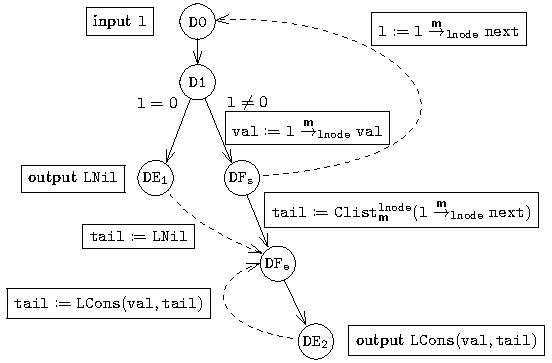
\includegraphics[scale=0.75]{chapters/figures/figClistCfg.pdf}
\caption{\label{fig:reconsProg}Reconstruction Program}
\end{subfigure}%
&
\begin{subfigure}[b]{0.50\textwidth}
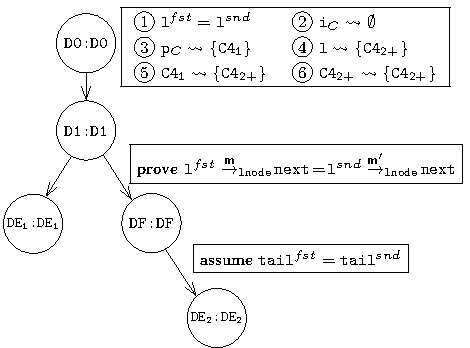
\includegraphics[scale=0.75]{chapters/figures/figClistProductCfg.pdf}
\caption{\label{fig:reconsPCFG}Recons-PCFG}
\end{subfigure}%
%&
%\begin{subfigure}[b]{0.17\textwidth}
%\includegraphics[scale=0.8]{figMallocPointsToGraph.pdf}
%\caption{\label{xxx}XXX}
%\end{subfigure}%
\\
\end{tabular}
\vspace{-8px}
\caption{\label{fig:recons}The reconstruction program and the recons-PCFG for {\tt Clist$^{lnode}_m({\tt l_{C}})$}. In \cref{fig:deconsProg}, {\tt D0} represents the unrolling procedure entry node, and the square boxes show the transfer functions of the unrolling procedure (\cref{eqn:clist}). The dashed edges represent a recursive function call. In \cref{fig:reconsPCFG}, the square box to the right of node {\tt D0:D0} contains the inferred invariants for this recons-PCFG.}
\vspace{-8px}
\end{figure}


The reconstruction
program and the recons-PCFG for our {\tt Clist} example
are shown in \cref{fig:recons}.
To check bisimulation
between the programs that deconstruct
${\tt Clist}_m^{{\tt lnode}}({\tt l}_C)$
and ${\tt Clist}_{m'}^{{\tt lnode}}({\tt l}_C)$, the recons-PCFG
correlates one unrolling of the first
program
with one
unrolling of the second program.
An unrolling of each reconstruction
program is based on the unrolling procedure in \cref{eqn:clist}.
Thus, the PC-transition correlations of both programs
are trivially obtained
by unifying the unrolling procedure with itself. A node
is created in the recons-PCFG that
encodes the correlation of the entries of the unrolling procedure in
both programs, we call this node the {\em recursive-node} in the
recons-PCFG, e.g., the
recursive node in \cref{fig:reconsPCFG} is {\tt R0:R0}. A recursive
call becomes a back-edge in the recons-PCFG that terminates at the
recursive-node.
A candidate
invariant at the recursive-node
is obtained by equating the pair of corresponding
{\tt l}$_C$ variables across the first and second
programs, i.e.,
${\tt l}^{fst}_C={\tt l}^{snd}_C$.
At the start of
both reconstruction
programs, ${\tt l}^{fst}_C={\tt l}^{snd}_C={\tt l}^{start}_C$
--- the
same ${\tt l}^{start}_C$ is passed to both reconstruction
programs, only the memory states $m$ and $m'$ are different.
The bisimulation check thus involves checking that
if the invariant
${\tt l}^{fst}_C={\tt l}^{snd}_C$
holds at the recursive-node,
then during one iteration of the unrolling procedure
in both programs:
\begin{enumerate}
\item The \underline{if} condition
({\tt l$^{fst}_C=0$}) in the first program
is equal to the corresponding \underline{if}
condition ({\tt l$^{snd}_C=0$}) in the
second program.
\item If the \underline{if} condition
evaluates to false in both programs, then
the observable values (that are used in the
construction of the list) are equal, i.e.,
$(({\tt l}^{fst}_C\neq 0)\land({\tt l}^{snd}_C\neq 0))\Rightarrow (\structPointer{{\tt l}^{fst}_C}{m}{\tt lnode}{val}=
\structPointer{{\tt l}^{snd}_C}{m'}{\tt lnode}{val})$.
\item If the \underline{if} condition
evaluates to false in both programs, then
the invariant holds at the beginning
of the unrolling procedure invoked through the
recursive call.
This involves checking equality
of the arguments to the recursive call, i.e.,
$(({\tt l}^{fst}_C\neq 0)\land({\tt l}^{snd}_C\neq 0))\Rightarrow \structPointer{{\tt l}^{fst}_C}{m}{\tt lnode}{next}
=
\structPointer{{\tt l}^{snd}_C}{m'}{\tt lnode}{next}$.
\end{enumerate}
The first check succeeds due to the invariant
${\tt l}^{fst}_C={\tt l}^{snd}_C$.
For the second and third checks, we additionally
need to reason that the memory objects
$\structPointer{{\tt l}^{fst}_C}{m}{\tt lnode}{val}$ and
$\structPointer{{\tt l}^{fst}_C}{m}{\tt lnode}{next}$ cannot
alias with the writes (in $m'$ in \cref{eqn:memstore})
to the newly allocated objects
${\tt p}_C\xrightarrow[]{m}_{\mathrm{\tt lnode}}{\tt val}$
and
${\tt p}_C\xrightarrow[]{m}_{\mathrm{\tt lnode}}{\tt next}$.
This aliasing information is captured using a points-to analysis,
described next in \cref{sec:pointsTo}.

Notice that a bisimulation check
between the reconstruction programs is significantly
easier than the top-level bisimulation check between \SpecL{}
and C programs: here,
the correlation of PC transitions is trivially
identified by unifying the unrolling procedure with itself, and
the candidate invariants
are obtained by equating each corresponding pair
of variables across
the two programs.

\subsubsection{Points-to Analysis}
\label{sec:pointsTo}
To reason about aliasing (as required during the bisimulation
check in \cref{sec:bisim}), we conservatively compute the
{\em may-point-to}
information for each program value using Andersen's algorithm \cite{andersen94programanalysis}.
The range of this computed
may-point-to function are {\em sets of region labels}, where
each region label identifies a set of memory objects.
The sets of memory objects identified by two distinct region
labels are necessarily disjoint. We write $p\pointsTo\{R_1,R_2\}$
to represent the condition that value $p$ may point to
an object belonging to one of the region labels $R_1$ or $R_2$ (but
may not point to any object outside of $R_1$ and $R_2$).

We populate the set of all region labels using the
{\em allocation
sites} of the program, i.e., PCs where a call to
{\tt malloc} exists, e.g., {\tt C4}
in \cref{fig:llAllocCIR} is an allocation site.
For each allocation site $A$, we create
two region labels: (1) the first region label, called $A_1$,
identifies the set of memory
objects that were allocated by the most recent execution of $A$. (2) The second
region label, called $A_{2+}$, identifies
the set of memory objects that were allocated by older (not the most
recent) executions of $A$.

For example, at the start of PC {\tt C7} in \cref{fig:llAllocCIR},
{\tt i}$_C\pointsTo{}\emptyset$,
{\tt n}$_C\pointsTo{}\{{\tt C4}_1\}$,
and {\tt l}$_C\pointsTo{}\{{\tt C4}_{2+}\}$.
Because the may-point-to analysis determines the
sets of objects pointed-to by {\tt n}$_C$ and {\tt l}$_C$ to
be disjoint ($\{{\tt C4_{1}}\}$ vs. $\{{\tt C4_{2+}}\}$), any
memory accesses through {\tt n}$_C$ and {\tt l}$_C$
cannot alias at {\tt C7} (for an access
offset that is within the bounds of
the allocation size `{\tt sizeof lnode}').

The may-point-to information is computed not
just for scalar program values ({\tt n}$_C$,
{\tt l}$_C$, ...) but also for each region label.
For region labels $A1_{r1}$, $A2_{r2}$, $A3_{r3}$:
$A1_{r1}\pointsTo{}\{A2_{r2},A3_{r3}\}$ represents
the condition that the values (pointers) stored
in objects identified
by $A1_{r1}$ may point to an object identified by
either $A2_{r2}$ or $A3_{r3}$ (but not to any object
outside $A2_{r2}$ and $A3_{r3}$).
In \cref{fig:llAllocCIR}, at PC {\tt C7}, we
get
${\tt C4}_{1}\pointsTo{}\{{\tt C4}_{2+}\}$ and
${\tt C4}_{2+}\pointsTo{}\{{\tt C4}_{2+}\}$.
The condition
${\tt C4}_{1}\pointsTo{}\{{\tt C4}_{2+}\}$
holds because the {\tt next} pointer of the object
pointed-to by ${\tt n}_C$ (which
is a ${\tt C4}_1$ object) may point to
a {\tt C4}$_{2+}$ object (e.g., object pointed-to
by {\tt l}$_C$).
Similarly, ${\tt C4}_{2+}\pointsTo{}\{{\tt C4}_{2+}\}$
says that a pointer within a {\tt C4}$_{2+}$ object
may point to a {\tt C4}$_{2+}$
object (but not to a {\tt C4}$_1$ object).

\subsubsection{Transferring points-to information to the recons-PCFG}
\label{sec:pointsToAsInvariants}
Recall that
in \cref{sec:recursiveEqToBisim},
we reduce a validity check of the condition
${\tt Clist}_m^{{\tt lnode}}({\tt l}_C)
\indEq{} {\tt Clist}_{m'}^{{\tt lnode}}({\tt l}_C)$
to a bisimulation check. Also, recall
that we discharge the bisimulation check through the construction
of a recons-PCFG that compares the unrolling procedure with itself (executing
on memory states $m$ and $m'$).
During this bisimulation check, we need to prove
that for each execution
of the unrolling procedure, $\structPointer{{\tt l}_C}{m}{\tt lnode}{\{val,next\}}$
and $\structPointer{{\tt l}_C}{m'}{\tt lnode}{\{val,next\}}$\footnote{Here, we use the symbol {\tt l}$_C$ to
refer to equal values {\tt l}$^{fst}_C$ and
{\tt l}$^{snd}_C$.} are equal.
To successfully discharge these proof obligations, it suffices
to show ${\tt l}_C$ cannot alias with the memory writes that
distinguish $m$ from $m'$.

Our points-to analysis on
the C program determines that at PC {\tt C5} (the start of
the product-CFG edge {\tt (S3:C5)$\rightarrow$(S3:C3)} across which the proof
condition is being evaluated),
the pointer to the {\em head}
of the list, i.e., ${\tt l}^{start}_C$
points to {\tt C4}$_{2+}$. It also determines that the distinguishing
writes modify memory regions belonging to {\tt C4}$_1$. 
Further, we get ${\tt C4}_{2+}\pointsTo{}\{{\tt C4}_{2+}\}$ at PC {\tt C5}.
However,
notice that these determinations only rule out aliasing of the list-head with
the distinguishing writes. We also need to confirm non-aliasing
of the internal nodes of the linked list with the distinguishing
writes.
For this, we need to identify a points-to invariant,
{\tt l}$_C\pointsTo{}\{{\tt C4}_{2+}\}$, at the recursive-node
of the recons-PCFG
(shown in \cref{fig:reconsPCFG}).
To see why {\tt l}$_C\pointsTo{}\{{\tt C4}_{2+}\}$ is
an inductive invariant at the recursive-node:
\begin{itemize}
\item (Base case) The invariant holds
at entry to the recons-PCFG (because it holds for ${\tt l}^{start}_C$).
\item (Induction step) If ${\tt l}_C\pointsTo{}\{{\tt C4}_{2+}\}$
holds at the start of an unrolling procedure,
it also holds at the start of a recursive call to the
unrolling procedure. This
follows from ${\tt C4}_{2+}\pointsTo{}\{{\tt C4}_{2+}\}$ (points-to information at PC {\tt C5}),
which ensures that {\tt l$_C$->next} may point to only ${\tt C4}_{2+}$ objects.
\end{itemize}

To identify this points-to invariant, we run
our points-to analysis (the same analysis that is run
on the C program) on the reconstruction programs (\cref{fig:reconsProg})
before
comparing them for equivalence. The boundary
condition for the points-to analysis at the
entry node of the reconstruction
program (e.g., {\tt R0} in \cref{fig:recons}) is based on
the results of the points-to analysis
on $C$ at the PC where the proof obligation is being discharged (e.g., {\tt C5}
in our \cref{fig:llAllocC}). The points-to invariants
at a node {\tt (R$^{fst}_i$,R$^{snd}_j$)} of a recons-PCFG are
derived from the results of the points-to analysis on the individual
reconstruction programs at nodes {\tt R}$^{fst}_i$ and {\tt R}$^{snd}_j$
respectively.

During proof obligation discharge (e.g., during the bisimulation
check on recons-PCFG), the points-to invariants are encoded as SMT constraints.
This allows us to successfully
complete the bisimulation proof on the recons-PCFG, and
consequently successfully discharge the
proof obligation
$\{\phi_{{\tt S3:C5}}\}\\({\tt S3\rightarrow S5\rightarrow S3}, {\tt C5\rightarrow C3}) \{l_{S}\indEq{}Clist^{{\tt lnode}}_{m}(l_{C})\}$ in \cref{tab:llproductInv}.
The points-to analysis is described more formally
in \cref{sec:pointsToFormal}.

%Thus, as a part of the invariant inference procedure on the product-CFG
%for the decomposition programs, we also run our points-to analysis on the
%product-CFG to identify points-to invariants at the product-CFG
%nodes.  This improves precision, as shown in the example discussed
%above.
\vspace{-5px}
\subsubsection{Proof discharge algorithm for Type III obligations}
\label{sec:cat3summary}

Before the start of an equivalence check, a points-to analysis is run on the $C$ IR once.
During the equivalence check,
to discharge a Type III proof obligation $P: {\tt LHS}\Rightarrow{\tt RHS}$ (expressed
in first-order logic), we first replace the recursive
values of program $S$ in the {\tt RHS}
with lifted C values, based on the equalities present in the {\tt LHS}, to
obtain $P_2$.
This is followed by decomposition and RHS-breaking of $P_2$.

Upon successful decomposition, we
obtain several smaller proof obligations.
To prove $P$, we require all these smaller proof
obligations to be provable. If any of these smaller proof obligations
is not provable, we are unable to prove $P$.  If we obtain a counterexample
to any of these smaller proof obligations, then that counterexample
also falsifies $P$.
Let $P_3$ represent any such smaller proof obligation.
{\tt RHS} of $P_3$, being
a decomposition clause,
must relate atomic expressions on the {\tt RHS}.
If $P_3$ relates two scalar values in the {\tt RHS}, then
it is a Type II proof obligation and can be discharged
using the algorithm in \cref{sec:cat2algo}.

If $P_3$ relates two lifted
expressions in
the {\tt RHS},
we check if the reconstruction
programs of the two lifted ADT values being
compared can be proven to be bisimilar (assuming that
{\tt LHS} of $P_3$ holds at the correlated entry nodes
in the recons-PCFG).
To improve
the bisimulation
check's precision, we transfer the points-to information of the $C$ program
(at the PC where the proof obligation is being discharged) to the entry
of the reconstruction programs. The same points-to analysis is ran on the
reconstruction programs to populate the points-to function at all PCs.

These queries
generated by a bisimulation check are discharged
by a recursive call to the proof discharge procedure.
The depth of these recursive calls to the
proof discharge procedure is determined by
the maximum {\em recursion nest depth} (similar
to loop nest depth) of the decomposition
program.

If the bisimilarity check succeeds, the proof procedure returns
true for $P$.
If the bisimilarity check fails,
we imprecisely return false for $P$ (without a counterexample).

Finally, if $P_3$ neither
relates two scalar values, nor relates two lifted expressions,
we attempt to prove that {\tt LHS} of $P_3$ imply {\tt false}.
If successfully disproven, we return false for $P$ with the counterexamples.
Otherwise, we imprecisely return false for $P$ (without a counterexample).

Please refer to {\tt Chapter \ThesisChapterAlgo{}} of the thesis for a
detailed discussion on the algorithms introduced in this section along
with their pseudo-code.